\documentclass{beamer}
 
\usepackage[utf8]{inputenc}
\usepackage{amsmath}
\usepackage{tabto}
\usepackage{graphicx}

 
%Information to be included in the title page:

\usetheme{Copenhagen}
\title[Linear Programming] %optional
{EE5327 Optimization}
 
 
\author[Anshika,Razat] % (optional, for multiple authors)
{Anshika Chaurasia \and \\Razat Shanker}
 
\institute[VFU] % (optional)
{
  
  EE18MTECH11017\\
  EE18MTECH11016
 
 }
 
\date[VLC 2013] % (optional)
{21 Feb 2019}
 
 
\begin{document}
 
\frame{\titlepage}

 
\begin{frame}
\frametitle{Linear Programming}

\begin{block}{Definition}
 Linear programming is a technique for the optimization of a linear objective function, subject to linear equality and linear inequality constraints.
\end{block}
\begin{center}

 $\min\limits_{x}\ c^Tx$
\begin{alignat*}{2}
  \\subject\hspace{0.1cm} to\hspace{0.1cm}  Ax &\le b
\\and\hspace{0.1cm} x &\ge 0   
\end{alignat*}

\end{center}




\end{frame}
 
 \begin{frame}
 \frametitle{Question 5.1}
 
Q. Graphically obtain a solution to the following
\begin{center}
   $\max\limits_{x}\ 6x_{1} + 5x_{2}$ 
\end{center}
 
 \\ with constraints
\begin{alignat*}{1}
 \\ x_{1} + x_{2} &\le 5
 \\ 3x_{1} + 2x_{2} &\le 12
 \\where \hspace{0.1cm} x_{1},x_{2} &\ge 0
 \end{alignat*}

\end{frame}
 
\begin{frame}
 \frametitle{Graphical Solution}
\begin{columns}
  \begin{column}{0.47\textwidth}
   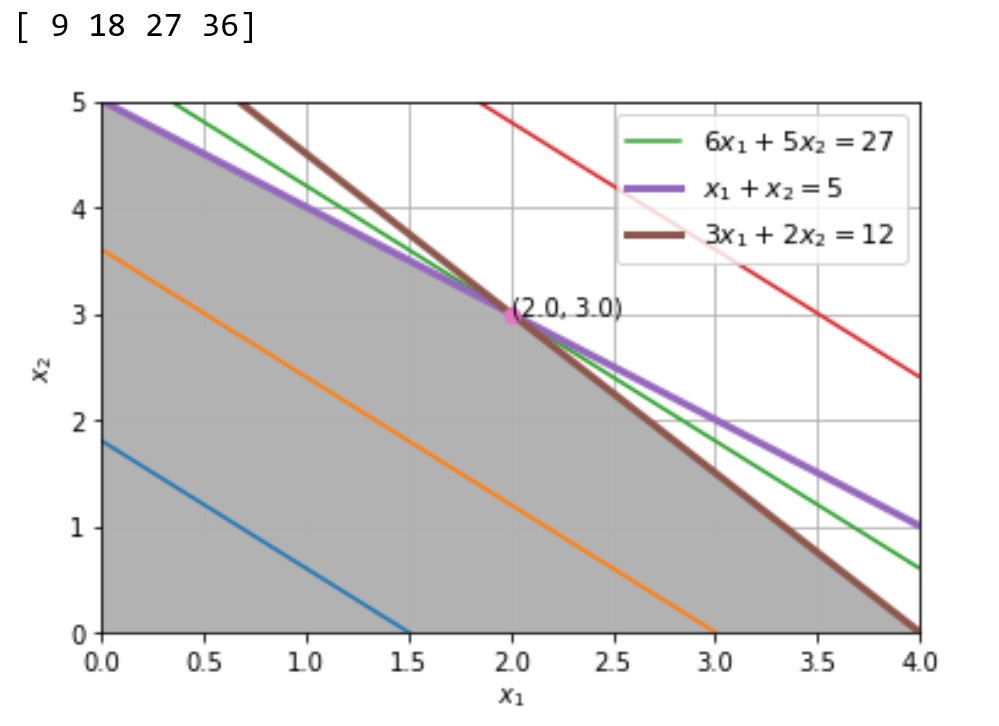
\includegraphics[width=5cm,height=5cm,angle=0]{g} 
  \end{column}
  \begin{column}{0.63\textwidth}
    \begin{table}[!ht]
   \centering
   \begin{tabular}{|c||c|} \hline
    \hline
     vertex of feasible \\ region & corresponding value \\& of  $\max\limits_{x}\ 6x_{1} + 5x_{2}$    \\ \hline
     (0,0) & 0 \\
     (0,5) & 25 \\
     (4,0) & 24 \\
     (2,3) & 27 \\ \hline
     \end{tabular}
    \end{table} 
  \end{column}
\end{columns}
  

\end{frame}

\begin{frame}
\frametitle{Question 5.2}
Q. Use cvxopt to obtain a solution to problem 5.1.  
 \begin{center}

 $\min\limits_{x}\ c^Tx$
\begin{alignat*}{2}
  \\subject\hspace{0.1cm} to\hspace{0.1cm}  Ax &\preceq b
\end{alignat*}

\end{center}
\[
c = 
\begin{bmatrix}
-6 
\\-5
\end{bmatrix}
,A = 
\begin{bmatrix}
1  &1 
\\3  &2
\\-1  &0
\\0  &-1
\end{bmatrix}
,B = 
\begin{bmatrix}
5
\\12 
\\0 
\\0  
\end{bmatrix}
\]
\end{frame}

\begin{frame}
\frametitle{Solution}
\begin{block}{Code:}

from cvxopt import matrix
\\from cvxopt import solvers \vspace{0.5cm}

\\A = matrix([ [1.0, 3.0, -1.0, 0], [1.0, 2.0, 0, -1.0] ])
\\b = matrix([ 5.0, 12.0, 0.0, 0.0 ])
\\c = matrix([ -6.0, -5.0 ])

\\sol = solvers.lp(c, A, b)

\\print(sol['x'])
 \end{block}
  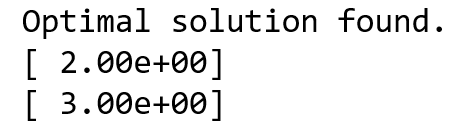
\includegraphics[width=4.5cm,height=2cm,angle=0]{Capture}
\end{frame}

\end{document}
